
このチュートリアルでは,Fig. \ref{fig:domain}に示した日本域を対象とした
現実大気実験を行う.
計算領域(ドメイン)の設定はTable \ref{tab:grids}のようになっている.

\begin{figure}[h]
\begin{center}
  \includegraphics[width=0.5\hsize]{./figure/domain.eps}\\
  \caption{計算領域.コンターは海岸線,カラーシェードは地形の高度を示す.}
  \label{fig:domain}
\end{center}
\end{figure}

\begin{table}[h]
\begin{center}
  \caption{実験設定の概略}
  \label{tab:grids}
  \begin{tabularx}{150mm}{|l|X|} \hline
    \rowcolor[gray]{0.9} 項目 & 設定 \\ \hline
    MPIプロセス分割 (東西 x 南北) & 3 x 3 (合計9プロセス) \\ \hline
    水平格子数 (東西 x 南北) & 180格子点 x 180格子点 \\ \hline
    鉛直層数                 & 36層                  \\ \hline
    水平格子間隔             & dx = dy = 7500m       \\ \hline
    積分期間 & 1999年5月5日 00UTC~12UTC (12時間積分) \\ \hline
    時間ステップ間隔 & 30 sec (1440 steps) \\ \hline
  \end{tabularx}
\end{center}
\end{table}

%-------------------------------------------------------%
\section{境界データの入手: AICS内部用、最終版では削ります}
%-------------------------------------------------------%

現実大気実験のシミュレーションを行う場合,SCALE本体に加えて境界値データが必要になる.
本チュートリアル用の気象場のデータ,日本領域の地形・土地利用のデータを\\
 \url{http://scale.aics.riken.jp/download/tutorial_data.tar.gz}\\
より入手し,チュートリアルの入力ファイル用ディレクトリ
\begin{verbatim}
  scale/scale-les/test/tutorial/data/
\end{verbatim}
の下に展開しておく.

以降の説明で\verb|${TOPDIR}|は,\verb|scale/scale-les/test/tutorial/|がある絶対PATHを指す.

\begin{verbatim}
  ${TOPDIR}/data/tutorial_data/input_atom/    <- 気象場データ
  ${TOPDIR}/data/tutorial_data/input_topo/    <- 地形データ
  ${TOPDIR}/data/tutorial_data/input_landuse/ <- 土地利用データ
\end{verbatim}
\verb|tutorial_data/|には,本チュートリアルに必要な最低限のデータのみが納めされているため,
その他の設定で実験を行う場合には別途,気象場,地形,および土地利用データが必要となる.


%-------------------------------------------------------%
\section{境界データの準備: 一般ユーザー用、公開時タイトル注意}
%-------------------------------------------------------%

現実大気実験のシミュレーションを行う場合,SCALE本体に加えて境界値データが必要になる。
境界値データとしては下記が必要である。
\begin{itemize}
\item 標高データ
\item 土地利用データ
\item 大気・地表面データ
\end{itemize}

ここでは、ユーザーが全球の任意の地域を対象とした計算できるよう、
標高データはUSGS(U.S. Geological Survey) のGTOPO30、
土地利用データはGLCCv2、
大気・地表面データはFinal Analysis の使い方を示す.


\subsubsection{地形データ: GTOPO30}

USGSのサイト\\
 \url{https://lta.cr.usgs.gov/GTOPO30}\\
からGTOPO30のデータをダウンロードする。
ダウンロードにはregistrationが必要である。

%以降の説明で\verb|${TOPDIR}|は,\verb|scale/scale-les/test/tutorial/|がある絶対PATHを指す.

つづく。





%-------------------------------------------------------%
\section{地形・土地利用データの作成:pp}
%-------------------------------------------------------%

ここでは,\ref{sec:source_code}節でダウンロードした\verb|tutorial_data|は,
\verb|${TOPDIR}/data/|の下に展開されていると想定している.

まず,ppディレクトリへ移動する.
ppでは現実実験のための地形データ、土地利用データを作成する.
\begin{verbatim}
 $ cd scale/scale-les/test/tutorial/pp
\end{verbatim}
ppディレクトリの中には,\verb|pp.conf|という名前の
コンフィグファイルが準備されている.
地球上でのドメインの位置や格子点数など、実験設定に合わせて,
適宜\verb|pp.conf|を編集する必要があるが,
チュートリアルでは,すでに編集済みの\verb|pp.conf|が
与えられているためそのまま利用する.
\verb|pp.conf|の設定の中で特に注意するべき項目は,\verb|PARAM_CONVERT|である.
\begin{verbatim}
 &PARAM_CONVERT
  CONVERT_TOPO = .true.,
  CONVERT_LANDUSE = .true.,
 /
\end{verbatim}
上記のように\verb|CONVERT_TOPO|と\verb|CONVERT_LANDUSE|が
\verb|.true.|となっていることが,
それぞれ地形と土地利用の処理を行うことを意味している.
詳細なコンフィグファイルの内容については,
Appendix \ref{app:namelist}を参照されたい.

次に,コンパイル済みのバイナリと入力データをppディレクトリへリンクする.
\begin{verbatim}
 $ ln -s ${TOPDIR}/bin/scale-les_pp ./
 $ ln -s ${TOPDIR}/data/tutorial_data/data/input_topo    ./
 $ ln -s ${TOPDIR}/data/tutorial_data/data/input_landuse ./
\end{verbatim}
今回は,Table \ref{tab:grids}に示されているように,
9つのMPIプロセスを使用する設定なので次のように実行する.
\begin{verbatim}
 $ mpirun -n 9 ./scale-les_pp pp.conf
\end{verbatim}
正常にジョブが終了すれば,\verb|topo_d01.pe######.nc|と\verb|landuse_d01.pe######.nc|というファイルがMPIプロセス数だけ,つまり9つずつ生成される(\verb|######|にはMPIプロセスの番号が入る).
それぞれ,ドメインの格子点に内挿された地形と土地利用の情報が入ってる.

処理内容のログとして,\verb|pp_LOG_d01.pe000000|という名前でログファイルも
出力されるので内容を確かめておくこと.
gpviewがインストールされていれば,次のコマンドによって作成された地形と土地利用データを
描画してチェックすることができる.
正しく作成されていれば,Fig. \ref{fig:domain}と同じように描かれる.
\begin{verbatim}
$ gpview topo_d01.pe00000*@TOPO --aspect=1
$ gpview landuse_d01.pe00000*@FRAC_LAND --aspect=1
\end{verbatim}


%-------------------------------------------------------%
\section{初期値・境界値データの作成:init}
%-------------------------------------------------------%

init では,SCALE計算に必要な初期値・境界値データを作成する.
まず,initディレクトリへ移動する.
\begin{verbatim}
 $ cd scale/scale-les/test/tutorial/init
\end{verbatim}

initディレクトリの中には,\verb|init.conf|という名前のコンフィグファイルが準備されている.
\verb|pp.conf|と同様に,実験設定に合わせて、この\verb|init.conf|を書き換える必要があるが、
チュートリアル用の\verb|init.conf|ファイルはTable\ref{tab:grids}の設定に
すでに合わせてある.
初期値・境界値データの作成には前節で作成した地形・土地利用データを利用する.
これは,下記のように,相対PATHを用いて参照するように設定されている.

\begin{verbatim}
&PARAM_TOPO
 TOPO_IN_BASENAME = "../pp/topo_d01",
/
&PARAM_LANDUSE
 LANDUSE_IN_BASENAME  = "../pp/landuse_d01",
/
\end{verbatim}
その他に\verb|init.conf|の設定の中で特に注意するべき項目は,
\verb|PARAM_MKINIT_REAL|である.

\begin{verbatim}
&PARAM_MKINIT_REAL
 BASENAME_BOUNDARY   = "boundary_d01",  <- 境界値データの出力名
 FILETYPE_ORG        = "NICAM-NETCDF",
 NUMBER_OF_FILES     = 2,               <- 読み込むファイルの数
 BOUNDARY_UPDATE_DT  = 21600.D0,        <- 入力データの時間間隔
 INTERP_SERC_DIV_NUM = 20,              <- 内挿計算用のチューニングパラメータ
/
\end{verbatim}

\verb|FILETYPE_ORG|は入力する気象場データのファイルフォーマットに
関するパラメータを設定しており,ここでは
NICAMモデルのnetcdf形式データのフォーマットで読み込むことを指定している.
詳細なコンフィグファイルの内容については,Appendix \ref{app:namelist}を参照されたい.

次に,コンパイル済みのバイナリをinitディレクトリへリンクする.
\begin{verbatim}
 $ ln -s ${TOPDIR}/bin/scale-les_init ./
\end{verbatim}
入力データはinitディレクトリの中に準備されている,\verb|"inputdata-link.sh"|を用いてリンクする.
\begin{verbatim}
 $ sh inputdata-link.sh
\end{verbatim}
としてスクリプトを実行することで,気象場の入力データがリンクされ,initディレクトリ内に下記のファイルがリンクされる.
このスクリプトにあるstart dateとend dateの設定項目を実験設定に対応するように編集するが、ここでは,start dateは1999/05/05 00:00:00,end dateは1999/05/06 00:00:00と設定している.もし,\verb|tutorial_data|を\verb|${TOPDIR}/data|以外の場所に展開している場合は,スクリプト内の
\verb|"dir"|の項目も適切なディレクトリに変更すること.下記ファイルにリンクが張れれば成功.
{\small
\begin{verbatim}

la_tg_00000.peall.nc    ms_qv_00000.peall.nc   oa_sst_00000.peall.nc  ss_tem_sfc_00000.peall.nc
la_tg_00001.peall.nc    ms_qv_00001.peall.nc   oa_sst_00001.peall.nc  ss_tem_sfc_00001.peall.nc
la_wg_00000.peall.nc    ms_tem_00000.peall.nc  ss_q2m_00000.peall.nc  ss_u10m_00000.peall.nc
la_wg_00001.peall.nc    ms_tem_00001.peall.nc  ss_q2m_00001.peall.nc  ss_u10m_00001.peall.nc
lsmask_00000.peall.nc   ms_u_00000.peall.nc    ss_slp_00000.peall.nc  ss_v10m_00000.peall.nc
lsmask_00001.peall.nc   ms_u_00001.peall.nc    ss_slp_00001.peall.nc  ss_v10m_00001.peall.nc
ms_pres_00000.peall.nc  ms_v_00000.peall.nc    ss_t2m_00000.peall.nc
ms_pres_00001.peall.nc  ms_v_00001.peall.nc    ss_t2m_00001.peall.nc

\end{verbatim} }

次に、陸面過程や放射過程のモデルを起動するためのパラメータファイルにリンクをはる.
\begin{verbatim}
 $ ln -s scale/scale-les/test/data/land/*  ./
 $ ln -s scale/scale-les/test/data/rad/*   ./
\end{verbatim}
上の行のリンクコマンドによって陸面過程のパラメータファイルがリンクされ,
下の行のコマンドによって放射過程のパラメータファイルがリンクされる.
準備が整ったら,9つのMPIプロセスを使用してinitを実行する.
\begin{verbatim}
 $ mpirun -n 9 ./scale-les_init init.conf
\end{verbatim}

正常にジョブが終了すれば,
\verb|boundary_d01.pe######.nc|と\verb|init_d01_00010713600.000.pe######.nc|というファイルが
MPIプロセス数だけ,つまり9つずつ生成される(\verb|######|にはMPIプロセスの番号が入る).
それぞれ,境界値データと初期値データが入ってるおり,境界値データには複数の時刻のデータが1つのファイルに含まれている.
初期値ファイルの名前のうち\verb|"00010713600.000"|の部分は,モデル内で算出された実験開始時刻を表している.

処理内容のログとして,\verb|init_LOG_d01.pe000000|という名前でログファイルも出力されるので内容を確かめておくこと.
gpviewがインストールされていれば,次のコマンドによって作成された地形と土地利用データを描画してチェックすることができる.
正しく作成されていれば,Fig. \ref{fig:init}と同じように描かれる.

\begin{verbatim}
$ gpvect --scalar --slice z=1500 --nocont --aspect=1 --range=0.001:0.015          \
         --xintv=10 --yintv=10 --unit_vect init_d01_00010713600.000.pe00*@QV      \
         init_d01_00010713600.000.pe00*@MOMX init_d01_00010713600.000.pe00*@MOMY
\end{verbatim}


\begin{figure}[h]
\begin{center}
  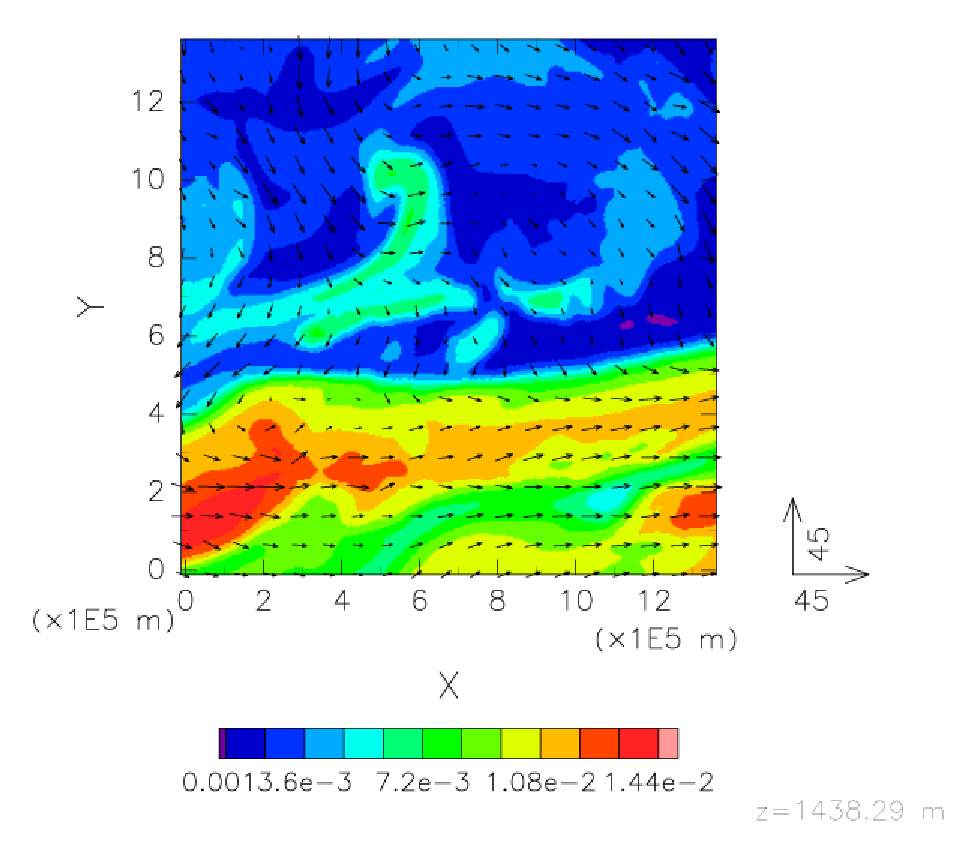
\includegraphics[width=0.7\hsize]{./figure/init_qv-momxy.eps}\\
  \caption{チュートリアル実験の初期場の様子:カラーシェードは高度1.5kmにおける比湿の分布,ベクトルは高度1.5kmにおける水平運動量フラックスを表している.}
  \label{fig:init}
\end{center}
\end{figure}


%-------------------------------------------------------%
\section{時間積分を行う:run}
%-------------------------------------------------------%

ここではいよいよSCALE-LESモデルを実行する.
まず,runディレクトリへ移動する.
\begin{verbatim}
  $ cd scale/scale-les/test/tutorial/run
\end{verbatim}


runディレクトリの中には,これまでと同様に\verb|run.conf|という名前のコンフィグファイルが準備されている.
チュートリアル用の\verb|run.conf|ファイルのドメインの位置や格子点数などはTable\ref{tab:grids}の設定に合わせてある.
モデル本体の実行には事前に作成した地形・土地利用データや初期値・境界値データを利用する.
これらのファイルを参照するために,
\verb|TOPO_IN_BASENAME|,\verb|LANDUSE_IN_BASENAME|,
\verb|RESTART_IN_BASENAME|,および\verb|ATMOS_BOUNDARY_IN_BASENAME|で
それぞれ場所を指定する.

\begin{verbatim}
&PARAM_TOPO
 TOPO_IN_BASENAME = "../pp/topo_d01",
/

&PARAM_LANDUSE
 LANDUSE_IN_BASENAME  = "../pp/landuse_d01",
/

&PARAM_RESTART
 RESTART_OUTPUT      = .false.,
 RESTART_IN_BASENAME = "../init/init_d01_00010713600.000",
/

&PARAM_ATMOS_BOUNDARY
 ATMOS_BOUNDARY_TYPE        = "REAL",
 ATMOS_BOUNDARY_IN_BASENAME = "../init/boundary_d01",
 ATMOS_BOUNDARY_USE_VELZ    = .true.,
 ATMOS_BOUNDARY_USE_QHYD    = .false.,
 ATMOS_BOUNDARY_VALUE_VELZ  = 0.0D0,
 ATMOS_BOUNDARY_UPDATE_DT   = 21600.0D0,
/

\end{verbatim}


\verb|run.conf|の設定の中で時間積分に関する設定は,\verb|PARAM_TIME|の項目にある.
\begin{verbatim}
&PARAM_TIME
 TIME_STARTDATE             = 1999, 5, 5, 0, 0, 0,
 TIME_STARTMS               = 0.D0,
 TIME_DURATION              = 12.0D0,
 TIME_DURATION_UNIT         = "HOUR",
 TIME_DT                    = 30.0D0,
 TIME_DT_UNIT               = "SEC",
 TIME_DT_ATMOS_DYN          = 7.5D0,
 TIME_DT_ATMOS_DYN_UNIT     = "SEC",

 ~~中略~~

/
\end{verbatim}

\verb|TIME_STARTDATE|は時間積分を開始する時刻を設定する項目で,チュートリアルでは1999年5月5日0時UTCと設定する.
\verb|TIME_DURATION|は積分期間を設定する項目で,ここでは12時間積分を行う設定になっている.
\verb|TIME_DT|,および\verb|TIME_DT_ATMOS_DYN|は,時間積分の間隔(時間ステップ間隔:DT = Delta Time)を設定する項目である.前者は移流計算,後者はそれ以外の力学過程の計算に関する時間積分間隔である.
SCALE-LESモデルでは,そのほかの物理過程についても細かく時間積分間隔を設定できるようになっている.


出力データに関する設定は\verb|PARAM_HISTORY|で行う.

\begin{verbatim}
&PARAM_HISTORY
 HISTORY_DEFAULT_BASENAME  = "history_d01",
 HISTORY_DEFAULT_TINTERVAL = 1800.D0,
 HISTORY_DEFAULT_TUNIT     = "SEC",
 HISTORY_DEFAULT_TAVERAGE  = .false.,
 HISTORY_DEFAULT_DATATYPE  = "REAL4",
 HISTORY_DEFAULT_ZINTERP   = .true.,
/
\end{verbatim}

\verb|HISTORY_DEFAULT_BASENAME|は出力するファイル名である.
\verb|HISTORY_DEFAULT_TINTERVAL|と\verb|HISTORY_DEFAULT_TUNIT|によってヒストリー出力時間間隔が設定される.
ここでは1800秒(30分)間隔での出力として設定されている.
この設定で,\verb|HISTITEM|として羅列された変数について出力される.
\verb|HISTITEM|では、オプション変数を加えることで、出力間隔を変数毎に変更したり、平均値を出力したりすることも出来る。
これらの説明は\ref{sec:output}を参照されたい.

\begin{verbatim}
&HISTITEM item="DENS" /           ! density (3D)
&HISTITEM item="MOMZ" /           ! vertical momentum (3D)
&HISTITEM item="MOMX" /           ! horizontal momentum-x (3D)
&HISTITEM item="MOMY" /           ! horizontal momentum-y (3D)
&HISTITEM item="RHOT" /           ! density * potential-temperature (3D)

&HISTITEM item="QV"   /           ! mixing ratio for vapor (3D)
&HISTITEM item="QHYD" /           ! mixing ratio for hydrometeor (3D)

&HISTITEM item="T"    /           ! temperature (3D)
&HISTITEM item="PRES" /           ! pressure (3D)
&HISTITEM item="U"    /           ! horizontal wind component-x (3D)
&HISTITEM item="V"    /           ! horizontal wind component-y (3D)
&HISTITEM item="W"    /           ! vertical wind component (3D)
&HISTITEM item="PT"   /           ! potential temperature (3D)
&HISTITEM item="RH"   /           ! relative humidity (3D)

&HISTITEM item="PREC" /           ! precipitation (2D)
&HISTITEM item="OLR"  /           ! out-going longwave radiation

&HISTITEM item="U10" /            ! horizontal wind component-x at 10m height(2D)
&HISTITEM item="V10" /            ! horizontal wind component-y at 10m height(2D)
&HISTITEM item="T2"  /            ! temperature at 2m height (2D)
&HISTITEM item="Q2"  /            ! mixing ratio for vapor at 2m height (2D)

&HISTITEM item="SFC_PRES"   /     ! pressure at the bottom surface (2D)
&HISTITEM item="SFC_TEMP"   /     ! temperature a the bottom surface (2D)
&HISTITEM item="LAND_SFC_TEMP" /  ! temperature a the bottom surface for land model (2D)
&HISTITEM item="URBAN_SFC_TEMP" / ! temperature a the bottom surface for urban model (2D)

\end{verbatim}


その他に実験で使用される物理過程の設定は,
\verb|PARAM_TRACER,PARAM_ATMOS,PARAM_OCEAN,PARAM_LAND,PARAM_URBAN|の項目に
記述されているので,実行前にチェックすること.
詳細なコンフィグファイルの内容については,Appendix \ref{app:namelist}を参照されたい.


次に,コンパイル済みのバイナリをrunディレクトリへリンクする.

\begin{verbatim}
  $ ln -s ${TOPDIR}/bin/scale-les ./
\end{verbatim}

また,前節と同様に陸面過程や放射過程のモデルを起動するためのパラメータファイルも
リンクしておく.

\begin{verbatim}
  $ ln -s scale/scale-les/test/data/land/*  ./
  $ ln -s scale/scale-les/test/data/rad/*   ./
\end{verbatim}
上の行のリンクコマンドによって陸面過程のパラメータファイルがリンクされ,
下の行のコマンドによって放射過程のパラメータファイルがリンクされる.
準備が整ったら,9つのMPIプロセスを使用してscale-lesを実行する.
\begin{verbatim}
  $ mpirun -n 9 ./scale-les run.conf < /dev/null >&log&
\end{verbatim}


実行にはおおよそ2時間を要するため,上記のように標準出力をファイルへ
吐き出すようにしてバックグラウンドで実行しておくと便利である.
計算が開始されれば,処理内容のログとして,\verb|"LOG_d01.pe000000"|ファイルが生成されるので,
例えば下記のようなコマンドで\verb|"LOG_d01.pe000000"|ファイルを参照すれば,
どこまで計算が進んでいるかチェックすることができる.
\begin{verbatim}
  $ tail -n 50 LOG_d01.pe000000
\end{verbatim}
正常にジョブが終了すれば,\verb|history_d01.pe######.nc|と\verb|restart_d01.pe######.nc|と
いう名前のファイルがMPIプロセス数だけ,つまり9つずつ生成される
(\verb|######|にはMPIプロセスの番号が入る).
historyファイルは実行結果のプロダクトであり,restartファイルは対応する時刻を開始時刻として
再計算を開始するための初期値ファイルである.

次節でhistoryデータを描画して結果を調べる方法を説明する.

%####################################################################################

